\documentclass[a4paper,12pt,twoside,final]{book}

\usepackage[top=43mm, bottom=44mm, left=41mm, right=32mm]{geometry}

\usepackage[toc,page]{appendix}
\usepackage[utf8]{inputenc}
\usepackage{amsfonts, amsmath, amsthm, amssymb, epsfig, graphicx, float}
% \usepackage[longnamesfirst,square,sort&compress, comma, super]{natbib}
% \usepackage[xindy,style=index]{glossaries}
\usepackage{palatino}
\usepackage{lipsum}
\usepackage{booktabs}
\usepackage[disable]{todonotes}
\usepackage{listings}
\usepackage{setspace}

\definecolor{grey}{rgb}{0.9,0.9,0.9}

\theoremstyle{definition}
\newtheorem{example}{Example}

\newcommand*\justify{%
  \fontdimen2\font=0.4em% interword space
  \fontdimen3\font=0.2em% interword stretch
  \fontdimen4\font=0.1em% interword shrink
  \fontdimen7\font=0.1em% extra space
  \hyphenchar\font=`\-% allowing hyphenation
}

% Configuration
	% Thesis title
	\newcommand{\thesisTitle}{Analyzing Privacy of Android Apps}
	% Thesis author
	\newcommand{\thesisAuthor}{GABRIELE PETRONELLA}
	% Author's previous degrees
	\newcommand{\authorDegrees}{B.S., Politecnico di Milano, Milan, Italy, July 2011}
	% Current degree (Thesis's degree)
	\newcommand{\thesisDegree}{Master of Science in Computer Science}

\PassOptionsToPackage{hyphens}{url}\usepackage[unicode,
			pdftex,
			plainpages=false,
			linktoc=all,
			hyperindex,
			breaklinks=true,
			citecolor=green,
			urlcolor=blue,
			hidelinks
		   ]{hyperref}
\hypersetup{
	pdftitle={\thesisTitle},
	pdfauthor={\thesisAuthor}
}

% Style
% !TEX root =  ../thesis.tex

\usepackage[top=43mm, bottom=44mm, left=41mm, right=32mm]{geometry}

\def\chapterautorefname{Chapter}
\def\sectionautorefname{Section}
\def\subsectionautorefname{Section}
\def\subsubsectionautorefname{Section}
\def\figureautorefname{Figure}
\def\tableautorefname{Table}

% Double spacing for text
\linespread{1.3}
% No square brackets in bibliography
\makeatletter
\renewcommand\@biblabel[1]{#1.}
\makeatother
% Bibliography style
% \renewcommand\bibname{}
% \renewcommand{\bibsection}{\section*{}}
% Single spacing list of abbreviations
% \renewcommand*{\glsgroupskip}{}
% Hyperref fix
\def\texorpdf #1#2{\texorpdfstring{#1{#2}}{#2}}

\usepackage[Lenny]{fncychap}

% Acronyms (to appear in the List of Abbreviations)
% \makeglossaries
% % !TEX root =  ../thesis.tex

% \newacronym{SMT}{SMT}{Simultaneous MultiThreading}
% \newacronym{OS}{OS}{Operating System}
% \newacronym{CPU}{CPU}{Central Processing Unit}
% \newacronym{I/O}{I/O}{Input/Output}
% \newacronym{GUI}{GUI}{Graphical User Interface}
% \newacronym{GPLv2}{GNU GPLv2}{GNU General Public License (version 2)}
% \newacronym{PID}{PID}{Process IDentifier}
% \newacronym{RSDL}{RSDL}{Rotating Staircase Deadline Scheduler}

\begin{document}
	\begin{titlepage}
	\topskip0pt
	\vspace*{\fill}
	\begin{spacing}{1.5}
	\begin{center}

		
\includegraphics[width=3cm]{images/logo-polimi.png}
		
		Politecnico di Milano

		\textit{Dipartimento di Elettronica, Informazione e Bioingegneria}

		\vspace{0.2cm}

		{LAUREA MAGISTRALE IN INGEGNERIA INFORMATICA}

		\noindent\rule{10cm}{0.4pt}
		
		\vspace{0.5cm}

		{\Large \thesisTitle}
		
	\end{center}
	\vspace{1.5cm}
	\begin{flushright}
		Thesis of:

		\textbf{Gabriele Petronella}

		\vspace{0.5cm}

		Matricola:

		\textbf{783759}
	\end{flushright}
	\begin{flushleft}
		Advisor (Politecnico di Milano):

		\textbf{Prof. Stefano Zanero}

		\vspace{0.5cm}

		Advisor (University of Illinois at Chicago):
		
		\textbf{Prof. Lenore D. Zuck}
	\end{flushleft}

	\vspace{0.7cm}

	\begin{center}
		{\footnotesize\fontfamily{pbk}\selectfont A.A. 2012 - 2013}
	\end{center}

	\end{spacing}
	\vspace*{\fill}
	\end{titlepage}

	\chapter*{}
		% !TEX root =  ../thesis.tex
\setcounter{page}{2}

\begin{flushright}
	\emph{To my family} \\
\end{flushright}

	\chapter*{Acknowledgements}
		% !TEX root =  ../thesis.tex

I want to thank Prof. Lenore D. Zuck for all the support and time she dedicated to me, helping me through this whole thesis work.
Then, I would like to thank want to tank Prof. Robert H. Sloan for the time he spent helping me in refining the scope of this thesis work.
Another thanks goes to Prof. Stefano Zanero for assisting me with his precious advice.

I finally want to thank all the people who shared with me this wonderful study and life experience in Chicago. I learned from this people more that I could ever possibly learn from books. Thank you for you awesomeness.

\begin{flushright}
GP
\end{flushright}


	% Optional Preface
	% \preface \label{preface}
	%	Blah
	
	\chapter*{Summary}
	\label{summary}
	In this thesis we present the design and the implementation of a tool to analyze privacy policies of Android applications, with the purpose of increasing the user's awareness about privacy-related concerns.
	The goal of this work is to produces a tool, targeted to users who wish to evaluate the compliance of arbitrary Android applications to their own privacy policies.
	The tool implements a semantic analyzer of privacy policies, able to extract relevant sentences from them and put them in relationship with the corresponding privacy-related permissions requested by applications.
	This work was inspired by the manual review of privacy policies of Android applications, and noticing how a common informal structure was evident across multiple documents.

	\chapter*{Ampio estratto}
	\label{chap:estratto}
	% !TEX root =  ../thesis.tex

Nel corso degli ultimi anni, le applicazioni per dispositivi mobili hanno avuto una grandissima crescita, sia in quantità, sia in importanza nelle nostre vite quotidiane.
Tale crescita sta segnando una vera e propria rivoluzione tecnologica, che porta ad importanti conseguenze nella vita di ciascuno di noi; mentre alcune di queste sono in buona parte positive e hanno l'effetto di semplificare e migliorare la vita degli utilizzatori di queste tecnologie, altre sono invece fonte di grandi preoccupazioni e introducono nuovi problemi da affrontare.

Nello specifico, il grande aumento in termini di potenzialità e penetrazione dei dispositivi mobili li ha resi una componente centrale della vita di molte persone; tali dispositivi contengono spesso un'incredibile quantità di dati sensibili del loro utilizzatore: email, messaggi, contatti, numeri di conto e molto altro.

Come, da chi e sotto quali circostanze queste informazioni possono essere accedute sono quindi domande che hanno assunto una fondamentale importanza.

In questa tesi cerchiamo la risposta a tali domande, analizzando due aspetti delle applicazioni per dispositivi mobili:

\begin{description}
  \item[permessi di sistema] limitazioni tecniche imposte dai sistemi operativi per dispositivi mobili, volte a limitare e controllare l'accesso a risorse sensibili, come ad esempio fotocamera, sensore GPS, rubrica e simili.
  \item[privacy policy] documenti legali che accompagnano le applicazioni per dispositivi mobili (e non) e che specificano - in linguaggio naturale - le modalità di trattamento dei dati personali, raccolti tramite l'applicazione.
\end{description}

Nello specifico, ci concentriamo sulle applicazioni per dispositivi Android, sistema operativo mobile sviluppato da Google.

Proponiamo quindi uno strumento di analisi automatica per applicazioni Android, che permette di mettere in relazione i due aspetti sopracitati per estrarre potenziali incongruenze.
Lo strumento, fruibile mediante applicazione web, permette di ricercare un'applicazione dal Play Store (lo store ufficiale di applicazioni Android) e di ottenere informazioni circa il suo livello di rispetto della privacy.

Dopo l'introduzione, nel \autoref{chap:SOA} esponiamo il contesto in cui ci poniamo per parlare di privacy di applicazioni, proponendo una formalizzazione di tale contesto. Presentiamo dunque i meccanismi di tutela della privacy forniti dai moderni sistemi operativi mobili, evidenziandone criticità e punti deboli.

Nel \autoref{chap:manual-analysis} presentiamo gli esperimenti preliminari che hanno permesso la realizzazione di uno strumento di analisi automatica, che coinvologono l'ispezione manuale di privacy policy e permessi Android.

Il \autoref{chap:automated-analysis} espone l'approccio utilizzato per analizzare in maniera automatica diversi aspetti delle applicazioni Android, con lo scopo di estrarre informazione circa il rispetto della privacy degli utilizzatori di tali applicazioni.

Il \autoref{chap:implem} è dedicato ai dettagli dell'implementazione espone le problematiche incontrate durante lo sviluppo dello strumento di analisi automatica seguite dalle soluzioni adottate. Nel \autoref{chap:results} esponiamo prima una metrica utilizzata per valutare il livello di affidabilità di un'applicazione, seguita dai risultati quantitativi derivanti dall'analisi di oltre 4000 applicazioni presenti sul Play Store. Seguono poi delle considerazioni qualitative sui risultati ottenuti. Le limitazioni e i possibili sviluppi dello strumenti di analisi automatica sono esposti nel \autoref{chap:conclusion}.

	\tableofcontents
	\listoftables
	\listoffigures
	% Remember to run makeglossaries thesis
		% \glsaddall
		% \printglossary[title=LIST OF ABBREVIATIONS]

	\chapter{Introduction}
		\label{chap:intro}
		% !TEX root =  ../thesis.tex

%%%%%%%%%%%%%%%%%%%%%%%%%%%%%%%%%%%%%%%%%%
During the last few years, mobile applications constantly grew in both number and importance in our everyday life. 

% \todo[inline]{Statistical data about mobile applications and device owners}

Such an impressive growth is marking a technology revolution, and, as many revolutions, it carries huge consequences affecting everyone's life. Some of these consequences lead to clear improvements, whereas others put under the spotlight some concerns that were not that relevant just a few years ago.

The increase in penetration and capabilities of mobile devices has turned them in something most people would find hard to separate from. Mobile devices nowadays typically hold a huge amount of information about their owners: email, messages, contacts, bank accounts, social network profiles, location information.

% \todo[inline]{Third-party applications}

How and under which circumstances such information can be disclosed has quickly become a concern.


This thesis work focuses on the first two steps discussed in the previous section.

The first step requires an in-depth analysis and comprehension of the most requested permissions, in order to identify the potential privacy concerns each one of them carries.

Once the permissions of interest have been identified we then perform a manual analysis in order to understand how privacy policies deal with the privacy concerns represented by them. The manual analysis will enable an automated process, which, given an arbitrary Android application published on the Play Store platform, retrieves its privacy policy and produces a human-readable report about the relationships between the permissions list and the analyzed legal document.

The final result will then allow a potential user to aggregate a large amount of privacy-related information in a quick and concise way, marking a clear step towards privacy awareness.

%%%%%%%%%%%%%%%%%%%%%%%%%%%%%%%%%%%%%%%%%%

The remainder of this thesis is organized as follows. Chapter 2 presents the manual analysis performed over privacy policies and permissions. Chapter 3 then describes the automatic analysis of Android apps, enabled by the results of Chapter 2. Chapter 4 presents the details of the implementation and of the tools used to support both manual and automated analysis. Chapter 5 presents a metric used for evaluating the compliance of Android applications w.r.t. their privacy policies, as well as quantitative results - measured with such metric - and qualitative results. Chapter 6 concludes this thesis, proposing possible further developments to the work done.
	\chapter{State of the Art}
		\label{chap:SOA}
		% !TEX root =  ../thesis.tex
\section{Privacy awareness context}
We now define the scope of this thesis, going through the main factors affecting privacy in mobile applications, and describing the existing relationships between them.

We identify three main factors to take into consideration:
\begin{itemize}
  \item permissions
  \item actions and behaviors
  \item privacy policies
\end{itemize}

\emph{Permissions} determine which data or services the app can access on the user's device, so they effectively define the maximum potential impact an application can have over the user's privacy: the fewer the permissions, the lower the risk. However, a recent study \cite{stickley} showed how, given only the \texttt{INTERNET} permission, an Android application was capable of stealing online account login credentials.
This highlights how permissions only represent a loose upper bound to the risk: even apps requesting one single permission can significantly affect the privacy of user.

% As discussed in \autoref{sec:android-permission-model}, permissions are declared upfront by Android applications and they are visible prior to the app's installation.

We define \emph{actions} as the minimum unit of work an application can do. Actions can be divided in two main categories

\begin{itemize}
  \item actions that cannot be performed without an explicit permission, and actions
  \item that do not require such explicit permission (e.g. impact local state of app)
\end{itemize}
The former category typically includes actions that have any impact on the device's security. Such actions are forbidden by the OS (\emph{Operating System}) by default, and are allowed only if specific permissions have been granted to the application. The latter usually represents actions not affecting the device's security, e.g. actions confined within the bounds of the application's internal logic.

We define \emph{behaviors} as sequences of one or more actions; such definition implies that some behaviors, namely those including actions from the first category, can occur only when specific permissions have been granted.


\begin{example}
\leavevmode
Let us a consider a game application that stores user's top scores and sends them over the Internet to a remote server.
We can break this app down into the following actions:
\begin{itemize}
  \item \texttt{save\_user's\_top\_scores} ($A_1$)
  \item \texttt{send\_top\_scores\_over\_the\_internet} ($A_2$)
\end{itemize} 
The sequence of $A_1$ and $A_2$ forms the behavior \texttt{store\_and\_send\_user's\_ top\_score\_to\_a\_ remote\_sever} ($B_1$).
$A_2$ requires the permission \linebreak \texttt{INTERNET} to be granted, whereas $A_1$ can always be performed.
This implies that $B_1$ can occur only if permission \texttt{INTERNET} is granted.
\end{example}

Thus, permissions enable actions, and actions can be composed to form behaviors. It is important to notice the cardinality of these relationships: one permission enables one or more actions; in turn, a behavior is enabled by one or more actions.

A many-to-many relationship exists between permissions and behaviors. Enabling one (or more) permissions can potentially enable one or more behaviors.
While some of these behaviors are expected, and even desirable, some others might result unexpected and potentially undesirable. 

\begin{figure}[tb]
\centering
     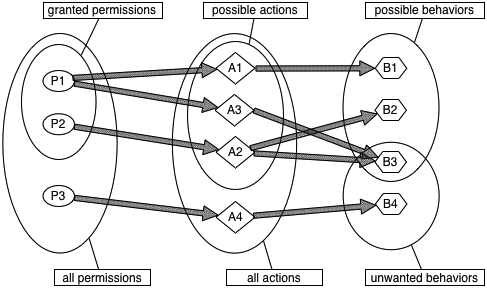
\includegraphics[width=0.9\textwidth]{images/context}
      \caption{Relationships between permissions, actions and behaviors}
      \label{fig:privacy-context}
\end{figure}

\autoref{fig:privacy-context} exemplifies this possible scenario: permission $P_1$ is required to enable action $A_1$ which in turn enables behavior $B1$. Similarly, permission $P_2$ enables action $A_2$ and consequently behavior $B_2$. Granting permissions $P_1$, however, also enables action $A_3$, and when combined with action $A_2$, an unwanted behavior $B_3$ may occur.

A practical instance of this scenario is the following:
\begin{example}
\leavevmode
\label{ex:unwanted-behavior}
\begin{itemize}
  \item the \texttt{READ\_PHONE\_STATE} permission enables the action \texttt{detect\_an\_ incoming\_phone\_call} ($A_1$), which enables the behavior \texttt{pause\_ the\_game\_when\_an\_incoming\_phone\_ call\_arrives} ($B_1$).
  \item the \texttt{INTERNET} permission enables the action \texttt{\justify send\_and\_receive\_ data\_over\_the\_Internet} ($A_2$), which enables the behavior \texttt{send\_ the\_user's\_top\_score\_to\_a\_remote \_server} ($B_2$).
  \item the \texttt{READ\_PHONE\_STATE} permission also enables the action \texttt{read\_the\_ user's\_phone\_ number} ($A_3$). The combination of actions $A_2$ and $A_3$ enables the behavior \\ \texttt{send\_the\_user's\_phone\_number\_to\_a\_remote\_server}($B_3$), which may be undesirable.
\end{itemize} 
\end{example}

Since the permission-based model has such shortcomings in properly restricting actions and avoiding unwanted behaviors, privacy policies are commonly provided together with the application, acting as a supplementary filter on the possible behaviors, telling the final users which of the possible behaviors the app is going to actually generate.

Coming back to Example 2, a privacy policy may explicitly state that the user's phone number is never collected nor accessed, promising the application will never perform \emph{A3}, and hence ruling out \emph{B3}. Nonetheless, nothing forbids an app to deviate from its policy.

\section{Scope of this thesis}
This thesis work focuses on the first two steps discussed in the previous section.

The first step requires an in-depth analysis and comprehension of the most requested permissions, in order to identify the potential privacy concerns each one of them carries.

Once the permissions of interest have been identified we then perform a manual analysis in order to understand how privacy policies deal with the privacy concerns represented by them. The manual analysis will enable an automated process, which, given an arbitrary Android application published on the Play Store platform, retrieves its privacy policy and produces a human-readable report about the relationships between the permissions list and the analyzed legal document.

The final result will then allow a potential user to aggregate a large amount of privacy-related information in a quick and concise way, marking a clear step towards privacy awareness.

%%%%%%%%%%%%%%%%%%%%%%%%%%%%%%%%%%%%%%%%%%

\section{Scope and goals of this thesis}
This thesis describes a methodology, supported by tools, that enables a user who installs an Android application to gain a better understanding of the app's capabilities, based on the permissions it requires and its privacy policy, and alerts the user to some of the (potentially) unintended consequences that the user grants the application by installing it.

\todo[inline]{Blablabla}
\section{Steps towards privacy awareness}
Given the general context of privacy awareness, we now identify a set of steps we intend to follow in our work, aiming at producing an increased users' awareness.

\begin{enumerate}
  \item Understanding permissions \hfill \\
    Previous studies \cite{Felt:2012:APU:2335356.2335360} show how permissions are rarely understood by users. Specifically users appear not be able to correlate a permission with the possible actions it enables, let alone the spectrum of possible behaviors derived from actions interleaving.

    The first step towards awareness is to analyze permissions and derive potential consequences. We are especially interested in permissions that directly affect privacy. As an example, the \texttt{READ\_PHONE\_ STATE} permission is typically requested by apps in order to be able to respond to phone events such as a incoming call, but it also enables the app to read the user's phone and IMEI numbers.

    Once permissions have been fully analyzed, one can then identify their  effect on the user's privacy.

  \item Correlating permissions and privacy policies \hfill \\
    The next step towards privacy awareness is to map each permission the app requests into its impact, as stated in its privacy policy.
    While privacy policies do not share a common defined structure, they do express similar concepts in similar ways, which allows us to extracting useful pieces of information from them. For example, an application requesting the \texttt{ACCESS\_FINE\_LOCATION} permission is very likely to be associated to a privacy policy containing expressions such as \emph{``GPS'', ``Location Services'', `Global Positioning System', etc}.

    This step takes into consideration each permission that enables an app to affect the user's privacy, with the final goal of building a dictionary of common expressions and patterns that associate the permission to natural language sentences in the privacy policy.

  \item Correlating apps behavior and privacy policies \hfill \\
    The final step is to monitor the app's actual behavior. Recalling Example \ref{ex:unwanted-behavior}, the application might never retrieve the user's phone number even though it requested such permission.

    On this basis we can advise the users about how well an application with respects the claims expressed in the privacy policy, and the actual actions taken by the app once installed and running on their phone.
\end{enumerate}

\begin{figure}[tb]
\centering
     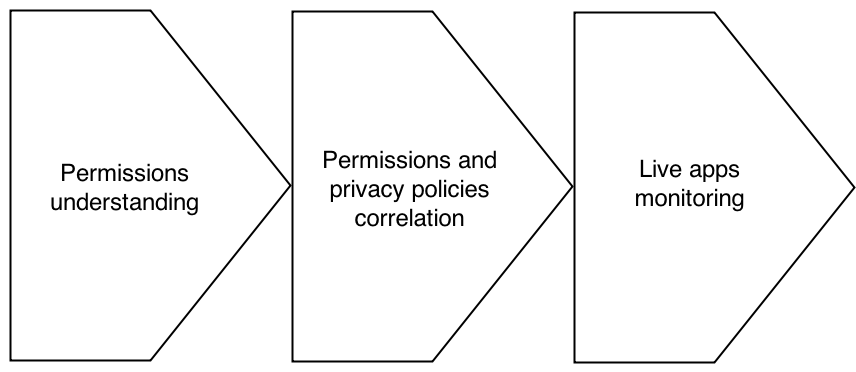
\includegraphics[width=0.8\textwidth]{images/awareness-steps}
      \caption{Privacy awareness steps}
      \label{fig:awareness-steps}
\end{figure}

%%%%%%%%%%%%%%%%%%%%%%%%%%%%%%%%%%%%%%%%%%

\section{Android OS Permission Model}
\label{sec:android-permission-model}
As explained in the Android Developer Guide, ``Android is a privilege-separated operating system, in which each application runs with a distinct system identity. [...]
Additional finer-grained security features are provided through a permission mechanism that enforces restrictions on the specific operations that a particular process can perform, and per-URI permissions for granting ad-hoc access to specific pieces of data. [...]
A basic Android application has no permissions associated with it by default, meaning it can not do anything that would adversely impact the user experience or any data on the device.''\cite{android-developer-guide}.
In order to access the protected features of the device the developer has to declare a list of permissions the application needs. This list is specified in the \texttt{AndroidManifest.xml}, a file containing application metadata, included by every Android application.

For example, an application that needs to send and receive data over the Internet would specify an \texttt{AndroidManifest} similar to the one in \autoref{lst:manifest}.

\begin{lstlisting}[
caption=Example of permission declaration in AndroidManifext.xml,
language=XML,
backgroundcolor=\color{white},
label=lst:manifest,
frame=single,
float,
basicstyle=\ttfamily\footnotesize
]
<manifest xmlns:android="http://schemas.android.com/res/android"
    package="com.example.anapp" >
    <uses-permission android:name="android.permission.INTERNET"/>
    ...
</manifest>
\end{lstlisting}

``At application install time, permissions requested by the application are granted to it by the package installer, based on checks against the signatures of the applications declaring those permissions and/or interaction with the user.
No checks with the user are done while an application is running: it either was granted a particular permission when installed, and can use that feature as desired, or the permission was not granted and any attempt to use the feature will fail without prompting the user.''\cite{android-developer-guide}

%%%%%%%%%%%%%%%%%%%%%%%%%%%%%%%%%%%%%%%%%%
\section{Related Work}
As discussed in \autoref{sec:android-permission-model}, permissions are granted at install time, meaning that a user is supposed to have reviewed the permissions the application requested and to have deemed them acceptable, before granting them altogether.

Such mechanism has been criticized for several reasons: first of all, recent studies \cite{Felt:2012:APU:2335356.2335360} \cite{Kelley:2012:CPI:2426020.2426027} show how users might not have complete understanding of the meaning and consequences of each permission in the list. The same studies also show how even experienced users are found not to pay attention to the permission list, most likely due to its verbosity and length. To further prove this last observation, in a recent experiment \cite{stickley} an ad-hoc application was developed and put on the Play Store; the application requested all possible permissions, enabling the researchers to steal personal data from the user, such as email addresses and phone numbers. The application received 1300 downloads over a 3-month period, without being advertised, and collected 1950 email addresses.

%%%%%%%%%%%%%%%%%%%%%%%%%%%%%%%%%%%%%%%%%%
	\chapter{Preliminary Experiments}
		\label{chap:manual-analysis}
		% !TEX root =  ../thesis.tex

\section{Overview}
\label{sec:overview}
In this chapter we will present the preliminary experiments we carried out, which involve the manual analysis of privacy policies and Android permission.
As we will see, this stage lays the foundation to a more sophisticated analysis, presented in \autoref{chap:automated-analysis}.

At the end of the chapter we will also anticipate some of the issues arising from this approach, as well as proposing possible workarounds.

%%%%%%%%%%%%%%%%%%%%%%%%%%%%%%%%%%%%%%%%%%
\section{Manual analysis}
In this section we present the preliminary manual steps that needed to be executed in order to enable an automated analysis.

\subsection{Permissions of Interest}
The first step in our research is to identify which of the permissions that an app can request have privacy related consequences.

Firstly, we are interested into discovering which are the most requested permissions in our domain of interest.
There are no official data released by Google, however we were able to retrieve empirical data with the use of
unofficial APIs \cite{play-store-unofficial-api}, discussed in greater details in \autoref{chap:implem}.

The Play Store platform divides apps in categories (such as \emph{Games}, \emph{Education}, \emph{Tools} and so on). We ran
an analysis on the most downloaded free apps for each category (a total of 4300 applications);
we retrieved the permission list for each one and aggregated the data. The top 20 requested permissions are shown in \autoref{tab:top20-permissions}.

\begin{table}[ht]
    \caption{TOP 20 REQUESTED PERMISSIONS IN FREE APPS}
    \label{tab:top20-permissions}
    \centering
    \begin{tabular}{clc}
        \toprule
            \#   & Permission & \% apps using it \\
            \midrule
                1  & INTERNET                       &   99.35\% \\
                2  & ACCESS\_NETWORK\_STATE         &   98.35\% \\
                3  & READ\_EXTERNAL\_STORAGE        &   92.35\% \\
                4  & WRITE\_EXTERNAL\_STORAGE       &   92.35\% \\
                5  & ACCESS\_WIFI\_STATE            &   85.47\% \\
                6  & READ\_PHONE\_STATE             &   78.39\% \\
                7  & WAKE\_LOCK                     &   59.65\% \\
                8  & VIBRATE                        &   32.79\% \\
                9  & GET\_ACCOUNTS                  &   32.79\% \\
                10 & ACCESS\_COARSE\_LOCATION       &   19.86\% \\
                11 & GET\_TASKS                     &   14.86\% \\
                12 & RECEIVE\_BOOT\_COMPLETED       &   13.88\% \\
                13 & ACCESS\_FINE\_LOCATION         &   9.93\%  \\
                14 & READ\_LOGS                     &   9.88\%  \\
                15 & MOUNT\_UNMOUNT\_FILESYSTEMS    &   6.93\%  \\
                16 & RECORD\_AUDIO                  &   5.95\%  \\
                17 & CHANGE\_WIFI\_STATE            &   4.98\%  \\
                18 & DISABLE\_KEYGUARD              &   4.95\%  \\
                19 & READ\_CONTACTS                 &   3.00\%  \\
                20 & WRITE\_SETTINGS                &   2.98\%  \\
        \midrule
            \multicolumn{3}{c}{\footnotesize \emph{Generated from 4300 apps on Nov 17, 2013}} \\
        \bottomrule
    \end{tabular}
\end{table}

The general list of permissions, however, includes permissions with no significant impact on privacy. We manually reviewed it to identify which permissions affect the user's privacy and how, obtaining a list of all of the permissions which enable actions that raises privacy concerns. For each permission, a list of enabled actions is provided, along with a discussion about the privacy concerns.

\begin{description}
    \item[INTERNET] \hfill
        \begin{description}
             \item[Actions enabled] \hfill
                \begin{itemize}
                     \item send data over the Internet
                     \item receive data over the Internet
                 \end{itemize} 
             \item[Privacy concerns]
                This permission is the most requested and also the most dangerous, privacy-wise, as it enables communication with remote servers over the Internet.
                Used in combination with other permissions, it allows the application to send any retrieved data to an arbitrary remote server.
             \item[Examples]
                An application can send any sensitive data retrieved thanks to other permissions over the Internet. For instance one can think of an application reading the user's phone number and sending it to a remote server, perhaps with the purpose of targeted phone advertisement.
                As described in a recent study \cite{stickley}, this permission can be dangerous by itself: a malicious application could collect sensitive data from the user (for example, a fake email client asking for username and password) and send them 
         \end{description} 
   
   \item[READ\_EXTERNAL\_STORAGE] \hfill
        \begin{description}
             \item[Actions enabled] \hfill
                \begin{itemize}
                     \item read files on the external SD card
                 \end{itemize} 
             \item[Privacy concerns]
                This permission allows to read files on an external SD card, so that anything stored in the external memory can be accessed by the app, including pictures, videos and data stored by other applications.
             \item[Examples]
                An application can retrieve all of the user's pictures stored on the SD card and send them to a remote server, violating the user's privacy.
         \end{description} 
    
    \item[WRITE\_EXTERNAL\_STORAGE] \hfill
        \begin{description}
             \item[Actions enabled] \hfill
                \begin{itemize}
                    \item write files on the external SD card
                    \item read files on the external SD card
                 \end{itemize} 
             \item[Privacy concerns]
                Despite the name, this permission implicitly enables also \\ \texttt{READ\_EXTERNAL\_STORAGE}, so the same privacy concerns apply.
         \end{description} 

    \item[ACCESS\_WIFI\_STATE] \hfill
        \begin{description}
             \item[Actions enabled] \hfill
                \begin{itemize}
                    \item access the \texttt{WifiManager}
                 \end{itemize} 
             \item[Privacy concerns]
                Accessing the \texttt{WifiManager} allows the app to read information about the WiFi network the device is connected to, including the current IP address.
             \item[Examples]
                A malicious application can track the user's location by estimating the WiFi network's location, as recent studies demonstrate \cite{Yang:2008:ELU:1339822.1339967}
         \end{description} 

    \item[READ\_PHONE\_STATE] \hfill
        \begin{description}
             \item[Actions enabled] \hfill
                \begin{itemize}
                    \item detect in-progress phone calls
                    \item read IMEI and IMSI identifiers
                    \item read the network provider information
                    \item read the user's phone number
                 \end{itemize} 
             \item[Privacy concerns]
                This is one of the most controversial permissions. While most applications request this permission in order to detect incoming phone calls, which is usually a legitimate use, it can also be used to retrieve sensitive information such as the user's own phone number.
             \item[Examples]
                An application can steal the user's phone number and sell it to advertisement companies for profit.

         \end{description} 

    \item[GET\_ACCOUNTS] \hfill
        \begin{description}
             \item[Actions enabled] \hfill
                \begin{itemize}
                    \item read the list of accounts from the Accounts Service
                 \end{itemize} 
             \item[Privacy concerns]
                The list of accounts consists of a list of usernames for each account associated with the device. For instance, the application might retrieve the email address associated with the user's GMail account.
             \item[Examples]
                Retrieving account's usernames can be the first step towards identity stealing. A malicious application can use this piece of information to break into a user's email account and access personal data.
         \end{description} 

    \item[ACCESS\_COARSE\_LOCATION] \hfill
        \begin{description}
             \item[Actions enabled] \hfill
                \begin{itemize}
                    \item know the (coarse) device location
                 \end{itemize} 
             \item[Privacy concerns]
                The coarse location is determined by the triangulation of GSM tower cells information and WiFi information. Although coarse, it can determine a user's location with a good level of accuracy, therefore representing a privacy concern.                
         \end{description}

    \item[GET\_TASKS] \hfill
        \begin{description}
             \item[Actions enabled] \hfill
                \begin{itemize}
                    \item know which tasks are running or recently run
                 \end{itemize} 
             \item[Privacy concerns]
                Allows an application to get information about the currently or recently running tasks. While not dangerous by itself, it can help in stealing information when combined with other permissions.
         \end{description} 

    \item[ACCESS\_FINE\_LOCATION] \hfill
        \begin{description}
             \item[Actions enabled] \hfill
                \begin{itemize}
                    \item know the (fine) device location
                 \end{itemize} 
             \item[Privacy concerns]
                The same concerns as coarse location apply.
         \end{description} 

    \item[READ\_LOGS] \hfill
        \begin{description}
             \item[Actions enabled] \hfill
                \begin{itemize}
                    \item read the low-level system log files
                 \end{itemize} 
             \item[Privacy concerns]
                Not particularly worrying by itself, but it enables the app to read everything other applications might have logged. If some application logs sensitive data, this permission will allow them to be read.
         \end{description} 

    \item[RECORD\_AUDIO] \hfill
        \begin{description}
             \item[Actions enabled] \hfill
                \begin{itemize}
                    \item record audio
                 \end{itemize} 
             \item[Privacy concerns]
                While this permission has legitimate uses, such as note taking or voice search, it is a potential tool for eavesdropping and recording sensible information. 
         \end{description}   

    \item[READ\_CONTACTS] \hfill
        \begin{description}
             \item[Actions enabled] \hfill
                \begin{itemize}
                    \item read the user's contacts data.
                 \end{itemize} 
             \item[Privacy concerns]
                The whole user's address book can be read. 
         \end{description}  

\end{description}

Table \autoref{tab:top-privacy-related-permissions} summarizes the privacy-related permissions we will consider in our analysis.

\begin{table}[ht]
    \caption{TOP PRIVACY-RELATED PERMISSIONS IN FREE APPS}
    \label{tab:top-privacy-related-permissions}
    \centering
    \begin{tabular}{clc}
        \toprule
            \#   & Permission & \% apps using it \\
            \midrule
                1  & INTERNET                       &   99.35\% \\
                2  & READ\_EXTERNAL\_STORAGE        &   92.35\% \\
                3  & WRITE\_EXTERNAL\_STORAGE       &   92.35\% \\
                4  & ACCESS\_WIFI\_STATE            &   85.47\% \\
                5  & READ\_PHONE\_STATE             &   78.39\% \\
                6  & GET\_ACCOUNTS                  &   32.79\% \\
                7  & ACCESS\_COARSE\_LOCATION       &   19.86\% \\
                8  & GET\_TASKS                     &   14.86\% \\
                9  & ACCESS\_FINE\_LOCATION         &   9.93\%  \\
                10 & READ\_LOGS                     &   9.88\%  \\
                11 & RECORD\_AUDIO                  &   5.95\%  \\
                12 & READ\_CONTACTS                 &   3.00\%  \\
        \midrule
            \multicolumn{3}{c}{\footnotesize \emph{Generated from 4300 apps on Nov 17, 2013}} \\
        \bottomrule
    \end{tabular}
\end{table}

\section{Relationship with privacy policy}
Now that we identified the permissions we are interested in, we want to see how each permission relates to the privacy policy, i.e. in which terms the privacy policy deals with permissions the app requested.

Our analysis involved an initial corpus of twenty policies. For each permission we went through each privacy policy of the corpus, manually extracting common pattern and terms.

The result of this manual investigation is a lookup table associating each permission with a list of common words or expressions used in the privacy policies to refer to the actions enabled by it.

\subsection{Example: Rovio's Privacy Policy}
We now illustrate what expressed in the previous section, taking a popular app's privacy policy as an example. The application in question is \emph{Angry Birds} by Rovio Entertainment Ltd. If we take the \texttt{ACCESS\_COARSE\_LOCATION} permission into consideration, we can find several parts of the privacy policy referring to it. Once such parts have been identified, the relevant words and expressions concerning the specific matter can be extracted. What follow are the relevant sections of Rovio's privacy policy concerning the user's location matter\cite{rovio}:

\begin{quote}
\emph{``Rovio or third parties operating the ad serving technology may use demographic and \textbf{geo-location} information (for more information regarding use of Location Data see below Section 3) as well as information logged from your hardware or device to ensure that relevant advertising is presented within the Service.''}
\end{quote}

\begin{quote}
\emph{``To the extent Rovio makes \textbf{location} enabled Services available and you use such Services, Rovio may collect and process your \textbf{\textbf{location}} data to provide \textbf{location} related Services and advertisements.''}
\end{quote}

\begin{quote}
\emph{``The \textbf{location} data is processed and stored only for the duration that is required for the provision of the \textbf{location} related Services.''}
\end{quote}

\begin{quote}
\emph{``Rovio may use, depending on the service (1)IP-based \textbf{location} based on the IP address presented by the end-user, (2) fine \textbf{geo-location} data based on coordinates obtained from a mobile device's \textbf{GPS} radio, or (3) coarse, network-based \textbf{geo-location} data based on proximity of network towers or the \textbf{location} of WiFi networks.''}
\end{quote}

\begin{quote}
\emph{``Your fine, \textbf{GPS-based} \textbf{geo-location} is not accessed without your consent.''}
\end{quote}

\begin{quote}
\emph{``Notwithstanding Rovio's partners who are providing location related parts of the Service, Rovio will not share your GPS geo-location with third parties without your consent.''}
\end{quote}

\begin{quote}
\emph{``To the extent Rovio makes available GPS geo-location to third parties in accordance with this Privacy Policy, it will be provided anonymously.''}
\end{quote}

\begin{quote}
\emph{``This includes, for example, collection of IP-based geolocation data to ensure that the product, service or features served comply with applicable laws of that nation.''}
\end{quote}

All of the above sentences are relevant to the matter of establishing what is the app expected behavior with respect to the user's location information. It is particularly interesting to observe a few characteristics of some of the cited sentences. Specifically Rovio's privacy policy states

\emph{``Your fine, \textbf{GPS-based} \textbf{geo-location} is not accessed without your consent.''}

This provides a false sense of assurance, since in Android application the consent has already been given at installation time, so the geo-location can always be accessed by the application without further notice to the user.

\subsection{Example: Halfbrick's Privacy Policy}
Similar examples can be found in many popular apps. Let us for instance consider the case of Halfbrick, a company most known for a game called Fruit Ninja. In the app's privacy policy we find

\emph{``Where you allow us access to such information, we may also collect information from your device such as your geographic location''}\cite{halfbrick}

Again, we can see how similar matters are mentioned similarly in different privacy policies, and also how again such a sentence provides false assurance: Android apps always have permissions granted upfront, so the phrase \emph{``Whenever you allow us''}, realistically means \emph{``Whenever the app is installed''} on an Android device.

\subsection{Lookup table example}
Based on this manual analysis, we built a look up table of permissions and the way they are referred to in policies. \autoref{tab:lookup-coarse-location} and \autoref{tab:lookup-record-audio} show examples of lookup table entries.

\begin{table}[tbh]
    \caption{ACCESS\_COARSE\_LOCATION LOOKUP TABLE}
    \label{tab:lookup-coarse-location}
    \centering
    \begin{tabular}{lp{6cm}}
        \toprule
            Permission   & Keywords \\
            \midrule
                \texttt{ACCESS\_COARSE\_LOCATION}  & \emph{``gps''}, \emph{``IP based location''}, \emph{``location''}, \emph{``location services''}, \emph{``geo-location''}, \emph{``geographic location''} \\
        \bottomrule
    \end{tabular}
\end{table}

\begin{table}[tbh]
    \caption{RECORD\_AUDIO LOOKUP TABLE}
    \label{tab:lookup-record-audio}
    \centering
    \begin{tabular}{lp{9cm}}
        \toprule
            Permission   & Keywords \\
            \midrule
                \texttt{RECORD\_AUDIO}  & \emph{``microphone''}, \emph{``record audio''}, \emph{``record voice''}, \emph{``audio''} \\
        \bottomrule
    \end{tabular}
\end{table}

\section{False positives}
\label{sec:false-positives}
Clearly, the main challenge of the approach we just described is reliably mapping privacy policies to permissions.
Due to the complexity of such challenge, the methodology occasionally suffers from false positives. For example, if we consider the sentence:

\emph{Merchandise can only be shipped to approved U.S. shipping locations.}

taken from the privacy policy of Shopkick (a popular shopping reward application, later discussed in \autoref{chap:results}), it is immediately evident to a human reader that, in this context, the word ``location'' does not refer to the collection of the user's location.
Most importantly, the sentence is not related with privacy matters at all and it should therefore not included in our mapping.

A few different approaches are possible in order to face the false positive issue.

A first possibility would be crowd-sourced human correction of tool results and improved NLP analysis of the text.
However, this would require a critical mass of users in order to produce significant results, thus we focused on an improved NLP analysis, which is likely to produce a more immediate impact.

From a technical point of view, ambiguities arise by the different meanings a word can have in different contexts. The intuition is to take the context into consideration, and widen the spectrum of our analysis.

Precisely examining the linguistic meaning of a sentence is a very hard task, arguably impossible in some instances. However, we can again take advantage of the particular domain we are looking at and consider the particular sentence structure typical of privacy policies.
Most sentence in the policies share a simple and straightforward structure that we can analyze more easily.

Instead of taking the whole linguistic structure into account, which would require an overly-complex NLP approach, we shift our attention to verbs only. The intuition behind this choice is that we can disambiguate the meaning of the terms we are looking for by considering the verbs that appear in the same sentences.

For example, ``location'' is ambiguous in the above sentence because of its double meaning of ``GPS location'' and ``physical location'', but we can easily disambiguate by looking for a derivation of the ``ship'' verb in the sentence, whose presence is likely to mark a false positive.

Similarly to what we have done with the lookup table, in this manual analysis step we then produce a ``false positive table'' for each permission, which we will then use during the automated analysis in order to exclude as many false positives as possible.
	\chapter{Automated analysis}
		\label{chap:automated-analysis}
		% !TEX root =  ../thesis.tex

%%%%%%%%%%%%%%%%%%%%%%%%%%%%%%%%%%%%%%%%%%
Once the lookup table has been constructed, it is then possible to proceed with an automated analysis of applications.
In this section we present the high level steps of the analysis, along with the challenges we face during this process, while the implementation details will be discussed in \autoref{chap:implem}.

\section{Privacy policy retrieval}
The first step is to retrieve the privacy policy, given an arbitrary application. This proved to be one significant challenge, for the following main reasons:
\begin{itemize}
    \item there is no legal requirement enforcing an Android application to have a privacy policy. Some applications simply do not provide one.
    \item there is no standard format for such documents. While the Play Store has a standard interface for providing a link to an app's privacy policy, the content of the link is arbitrary and completely at the discretion of the developer.
    \item some application developers do not provide a link to the privacy policy in the Play Store.
\end{itemize}

When present, the \emph{Privacy Policy} link in the Play Store interface can be followed to access the actual document, which can then be fetched in order to perform semantic analysis over it, as discussed in \autoref{sec:privacy-policy-analysis}.

For the purposes of this thesis, we limit our search for the privacy policy to the Play Store web interface. If the developer provided a privacy policy link, it is followed and analyzed, otherwise the search simply fails. This is a known limitation of this approach.

\section{Permissions retrieval}
The next step of the analysis involves retrieving the permissions list of an arbitrary Android application. This is a much easier task than retrieving the privacy policy, since every Android application is guaranteed to declare the requested permissions in a uniform format. The main challenge of this step is the implementation, due to the lack of official APIs to retrieve the desired information. Details of the solution are presented \autoref{chap:implem}.

\section{Privacy policy analysis}
\label{sec:privacy-policy-analysis}
Once the privacy policy document and the permissions list are both available, we can proceed with the semantic analysis.

First, the document is broken down into semantic sections, such as paragraphs and sentences.
Second, the keyword and expressions contained in the lookup table of each permission are matched against each section.
For each permission, the relevant matching sentences are then collected.

As discussed in \autoref{sec:false-positives}, we then identify false positive matches, i.e. the ones including verbs in the ``false positive table'', and exclude them from the final result set.

Such results are then presented to the final user, as discussed in the next section.

\section{User interface}
The results are made available to the user via a web interface. The interface allows the user to search for an arbitrary application on the Play Store; the permissions list and the privacy policy are then automatically retrieved, whenever possible.
The user has then the ability of selecting a specific permission, and a list of relevant sentences are extracted by the privacy policy and presented to them, along with an accurate description of the permission itself.

Such an interface allows the user to quickly evaluate the privacy-related risks of an Android application, by highlighting the relevant sections of the privacy policy and by providing useful information about sensible permissions.

%%%%%%%%%%%%%%%%%%%%%%%%%%%%%%%%%%%%%%%%%%
\section{Example}
We now present an example, in order to better summarize the steps discussed in the previous section.
\autoref{fig:example-search} shows the search interface: in the example we are searching for the game \emph{Angry Birds} and, as we type, a list of suggestions is dynamically computed by live-querying the Play Store, and presented to the user.

\begin{figure}[t]
\centering
     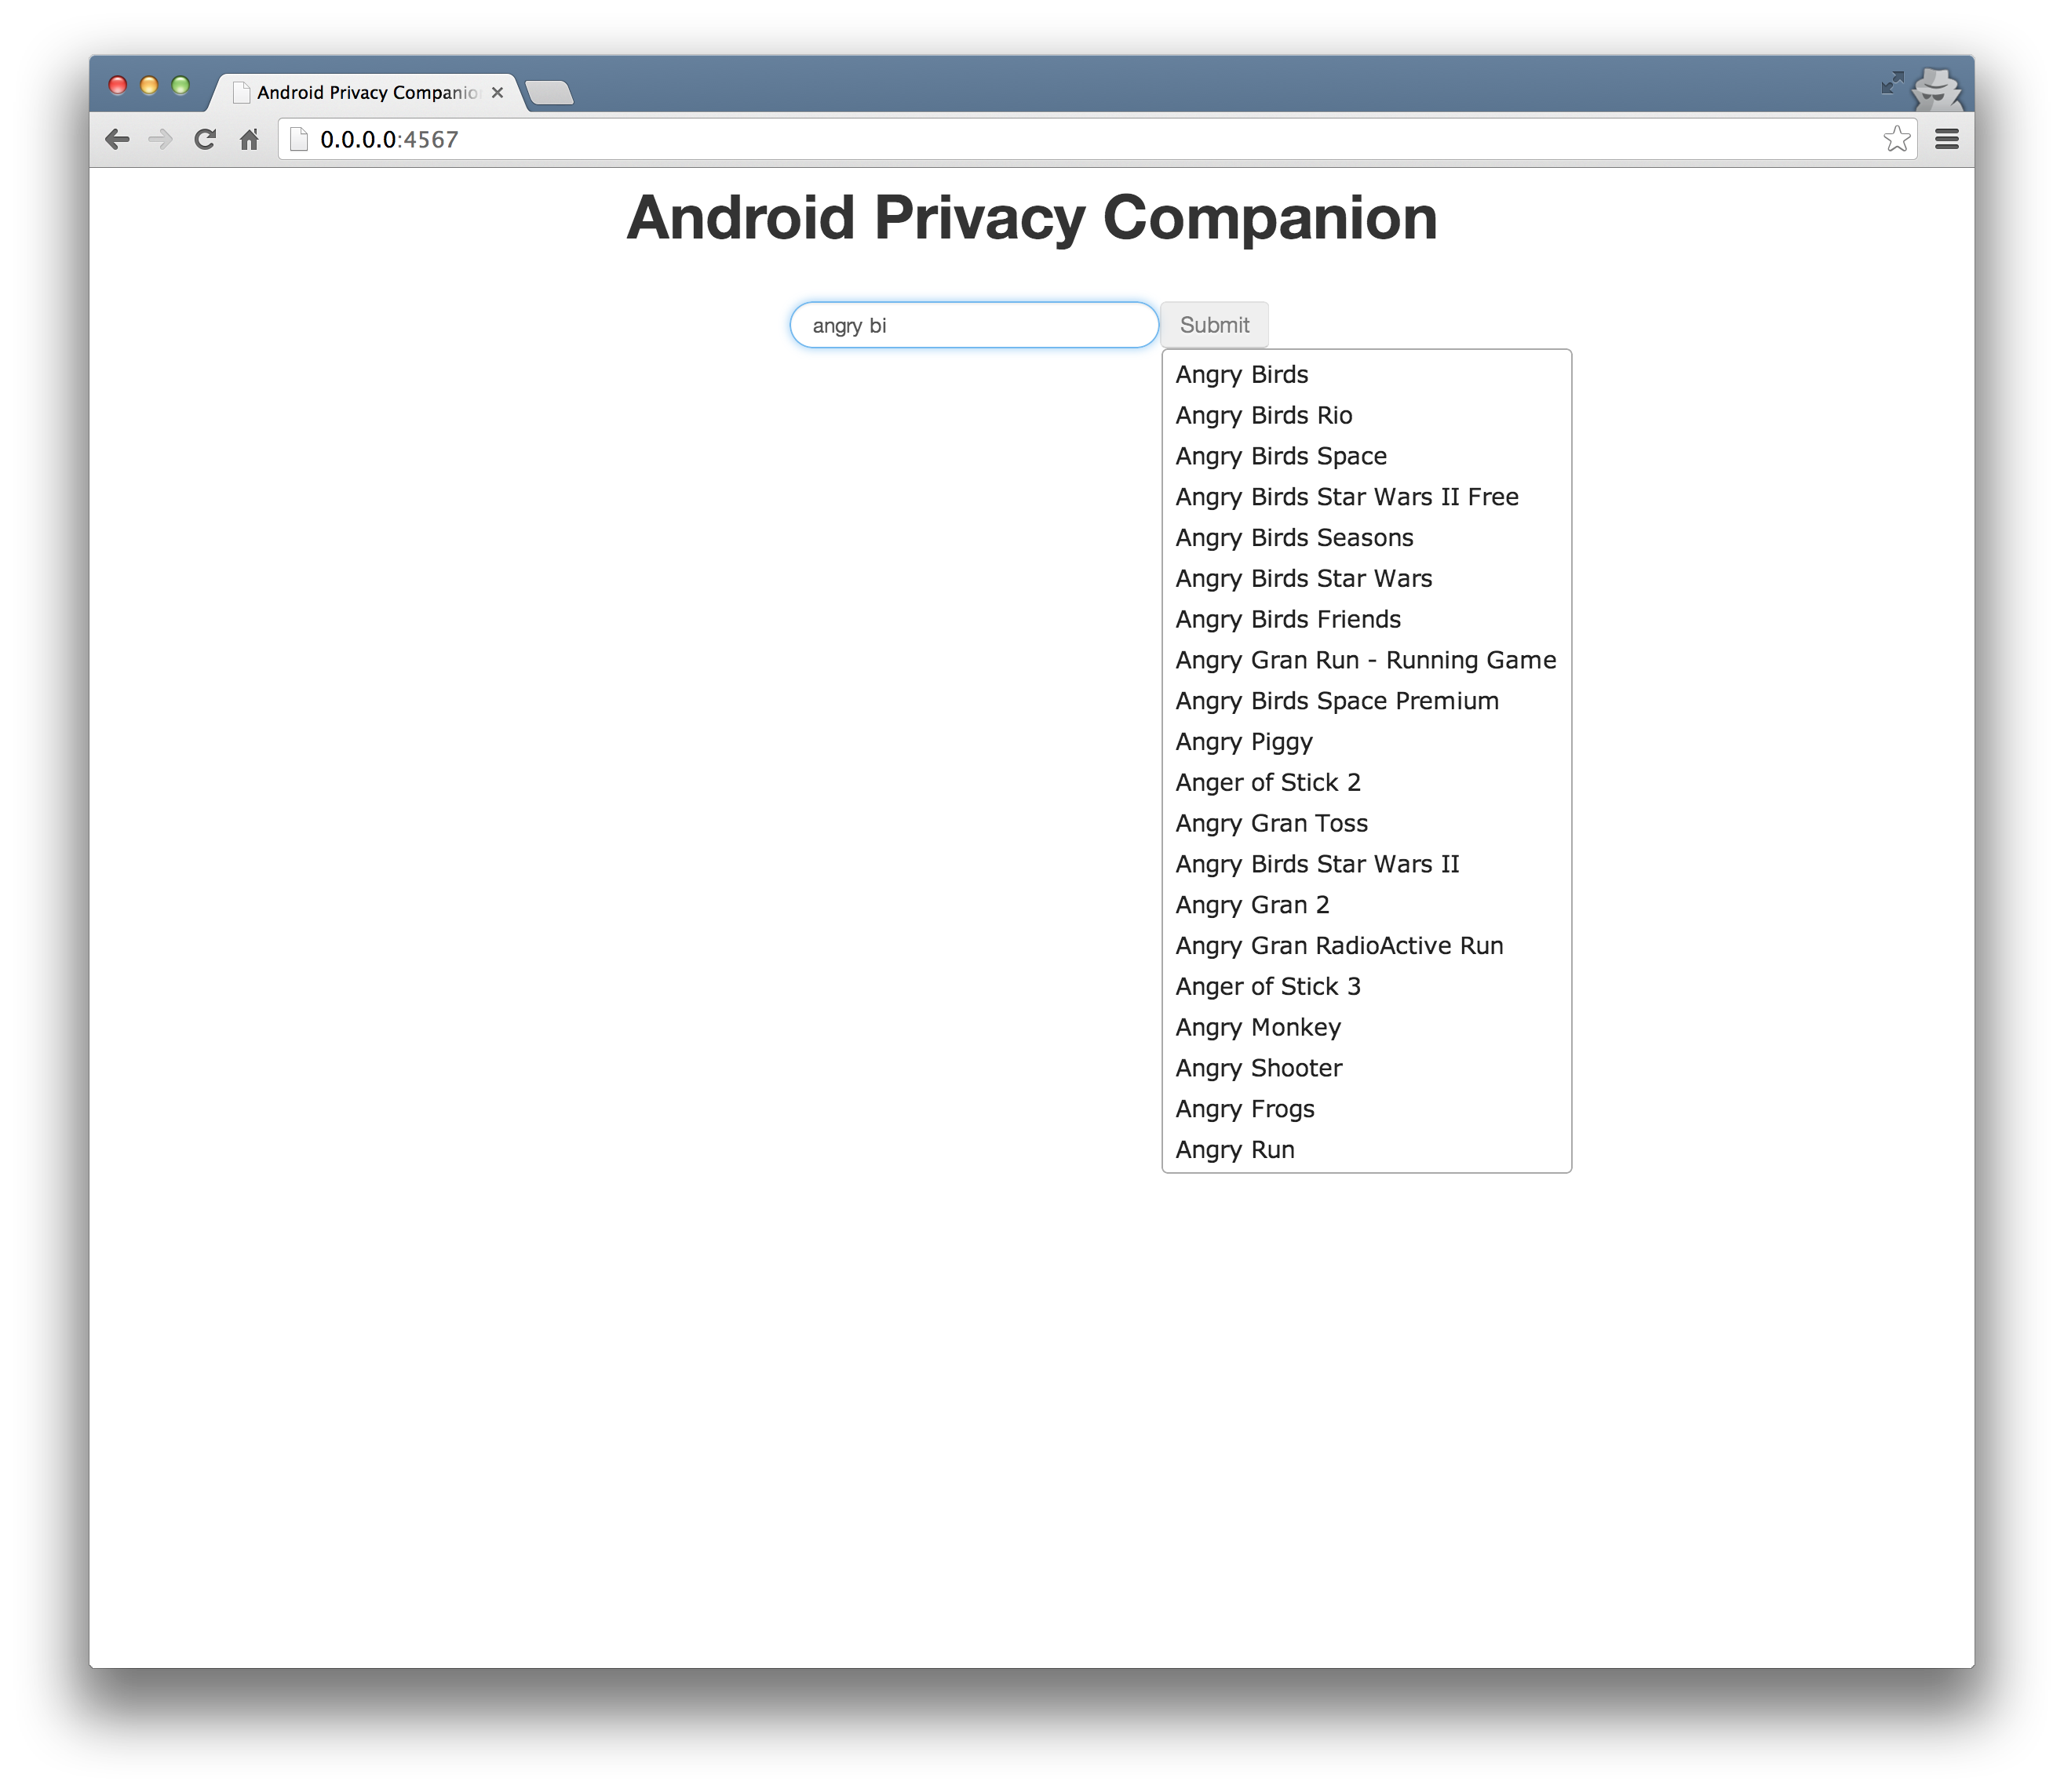
\includegraphics[width=.8\textwidth]{images/example-search}
      \caption{Search interface}
      \label{fig:example-search}
\end{figure}

Once the application has been selected from the list, the permissions list and the privacy policy are automatically retrieved and displayed.
The user can then select one of the permissions requested by the application in order to see all of the relevant sections of the privacy policy.

In \autoref{fig:example-permission-selected} the user selected the \texttt{ACCESS\_COARSE\_LOCATION} permission and a list of relevant sentences is displayed right under the permission description.

\begin{figure}[b]
\centering
     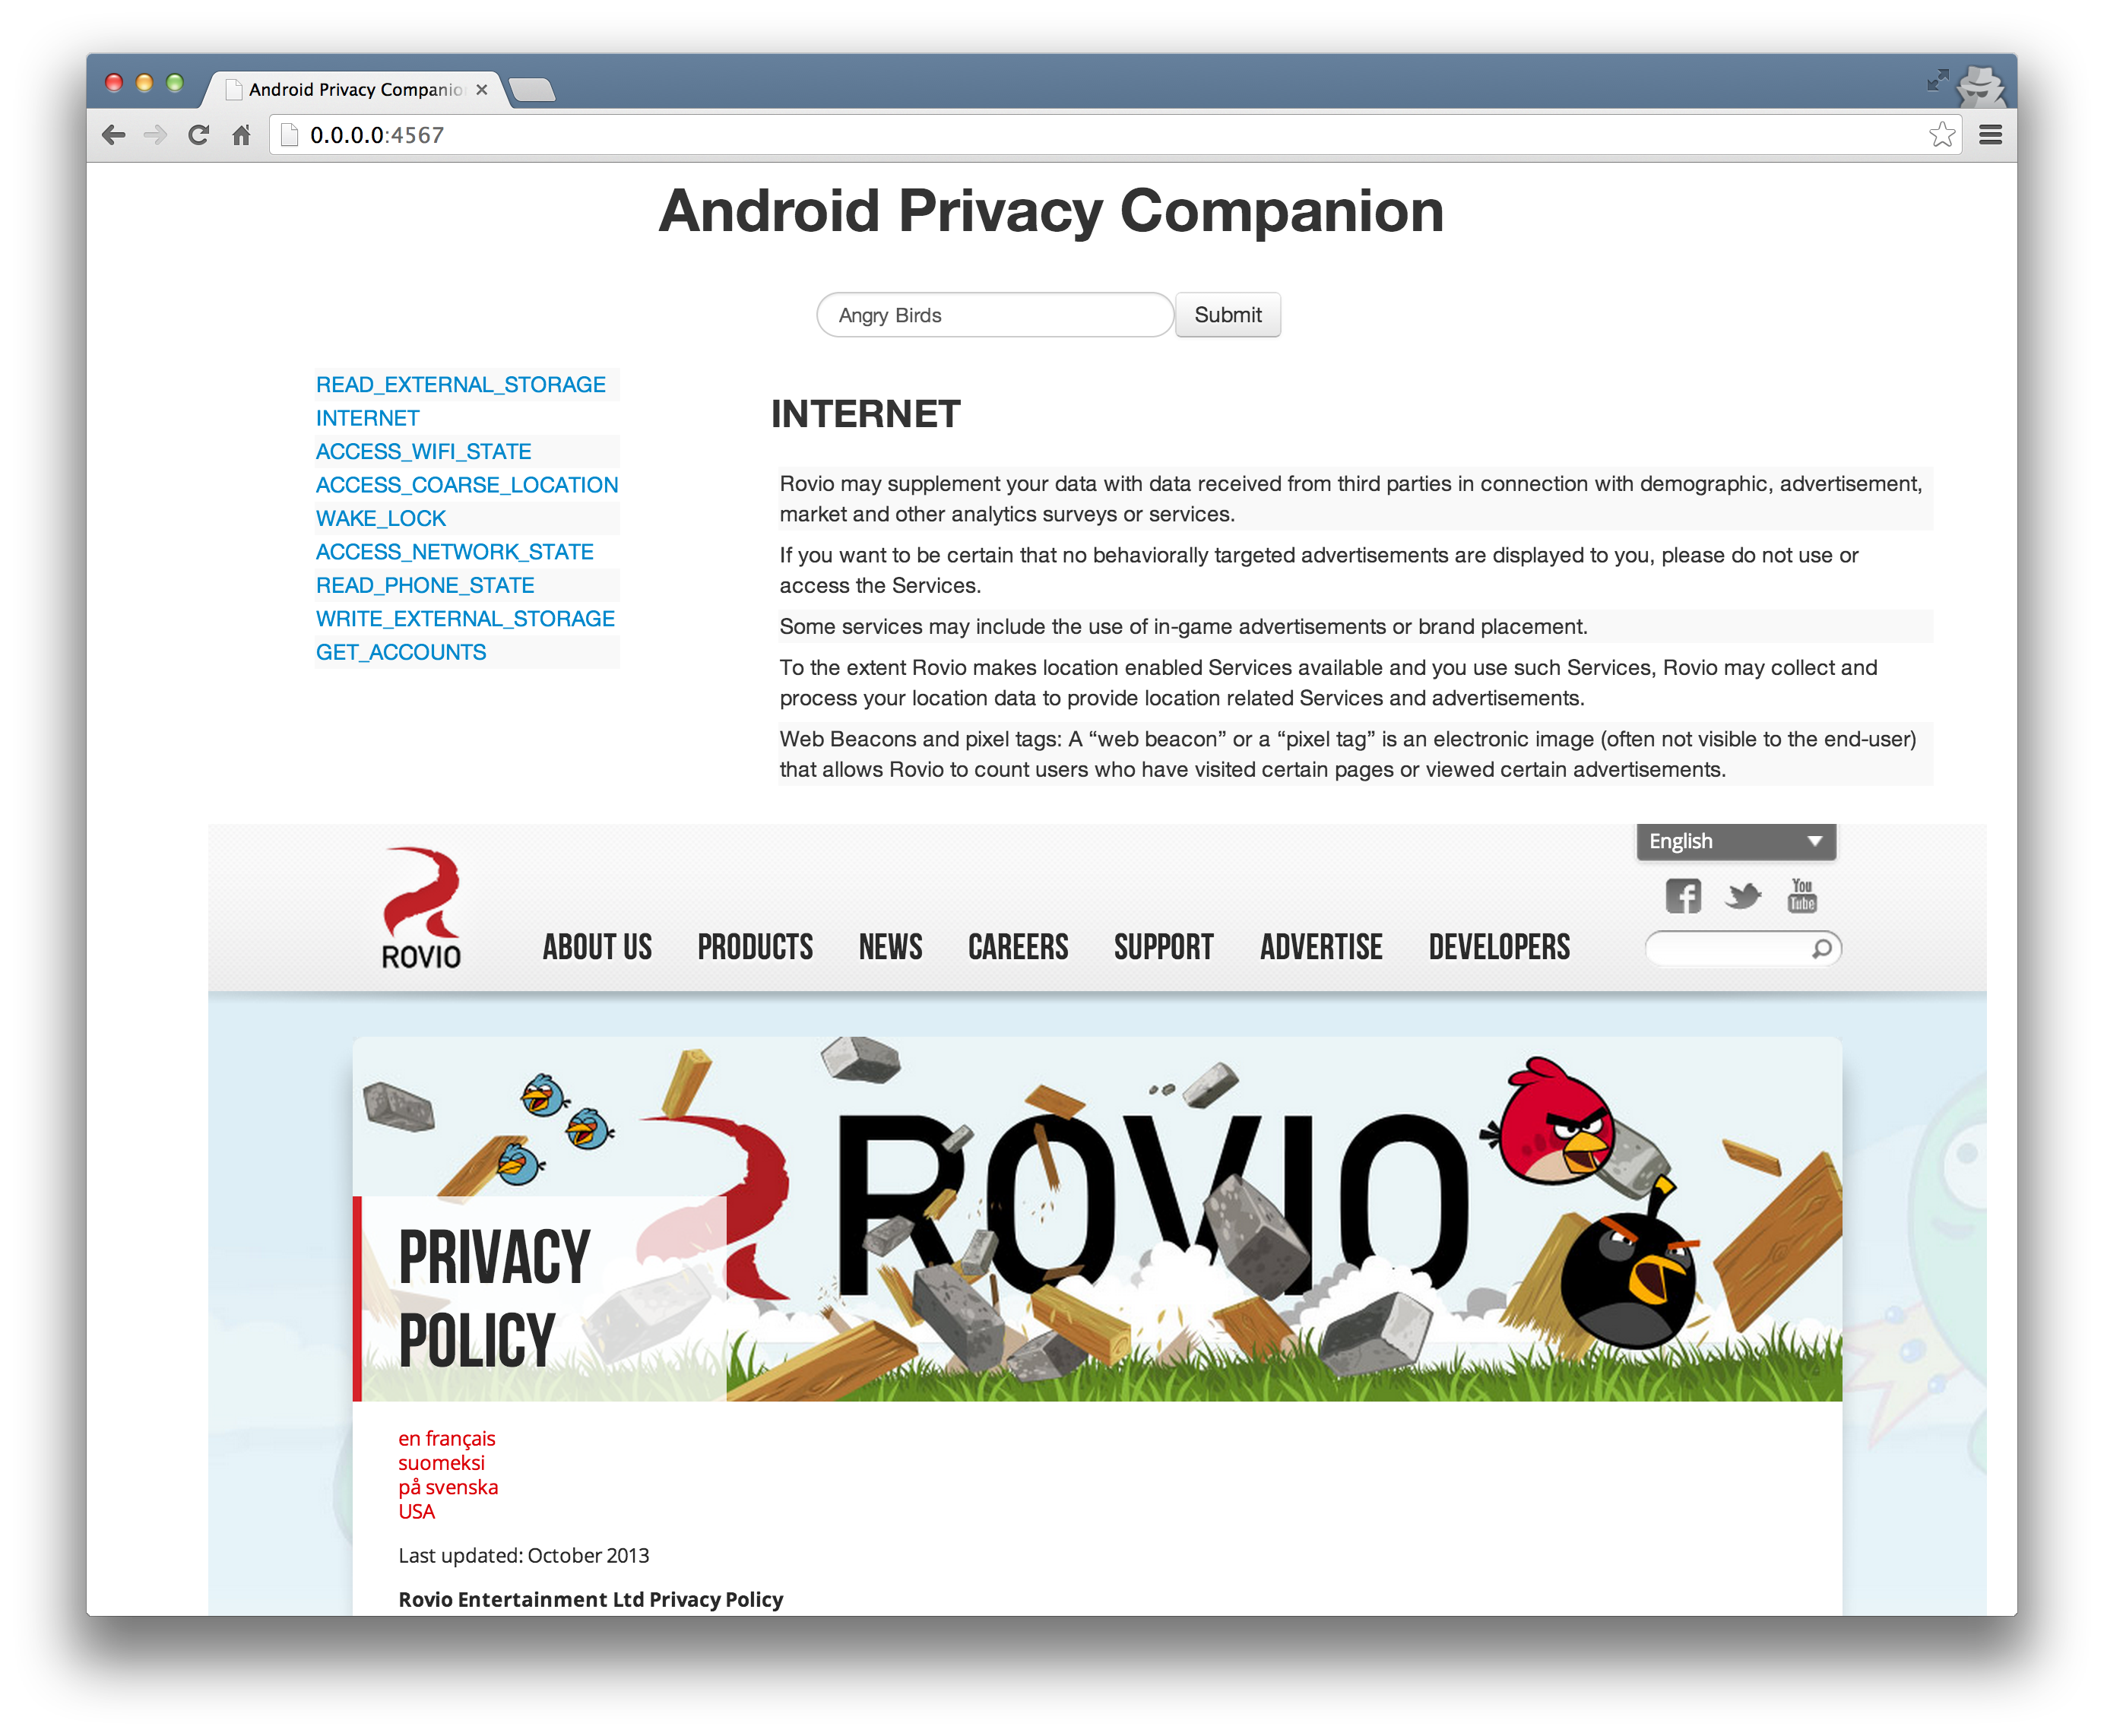
\includegraphics[width=.8\textwidth]{images/example-permission-selected}
      \caption{Permission display interface}
      \label{fig:example-permission-selected}
\end{figure}
	\chapter{Implementation}
		\label{chap:implem}
		% !TEX root =  ../thesis.tex
In this chapter we present the details of the implementation. We first describe the data collection process, for privacy policies and permissions; we then discuss how the collected data were subsequently analyzed, preprocessed and selected. Finally, we present the implementation of the algorithms discussed in the previous chapter.

%%%%%%%%%%%%%%%%%%%%%%%%%%%%%%%%%%%%%%%%%%
\section{Permissions collection}
\label{sec:permissions-collection}
As discussed in \autoref{sec:android-permission-model}, Android apps are required to declare upfront a list of all the permissions they need. Such list is stored in the \texttt{AndroidManifest.xml} file of each app. At installation time the user is able to review the permissions and decide whether to grant them or not.

Due to the lack of public official API for retrieving the permissions list, we first attempted to retrieve it through the Play Store web interface.

From a programmatic point of view, however, some issues arise. First of all, the permissions presented to the user are in a natural language format, whereas the permissions in the \texttt{AndroidManifest.xml} file are expressed with a canonical name. For instance the permission \texttt{READ\_ EXTERNAL\_STORAGE} correspond to the natural language description \emph{``modify or delete the contents of your USB storage''}.
This would require an extra processing step to map the natural language description back to the corresponding permission.

Secondly, and most importantly, the permission list is accessible from the web interface only after pressing the `install' button, and this step is allowed only from a registered Google account with at least one Android device registered.

While these issues can be overcome, they added unexpected complexity to this step, and therefore an alternative path was explored.

As mentioned above, Google does not provide an official API for retrieving applications metadata, such as the permission list. However an unofficial Python implementation exists and is publicly available \cite{play-store-unofficial-api}. There also exists another open-source project \cite{play-store-crawler}, based on the unofficial API, featuring the ability of performing search queries, downloading apps and retrieving apps permissions.

Thank to the use of the unofficial API, the issues mentioned above were solved and we were able to retrieve the permissions from an arbitrary app available on the Play Store.

%%%%%%%%%%%%%%%%%%%%%%%%%%%%%%%%%%%%%%%%%%
\section{Privacy Policy collection}
\label{sec:pp-collection}
Automatically retrieving a privacy policy document for an arbitrary Android app is a much harder task than retrieving its permission list.

Whenever present, the Privacy Policy link appears in the \emph{Additional Information} section on the Play Store web interface, as shown in \autoref{fig:play-store-privacy-link}.

\begin{figure}[tb]
\centering
     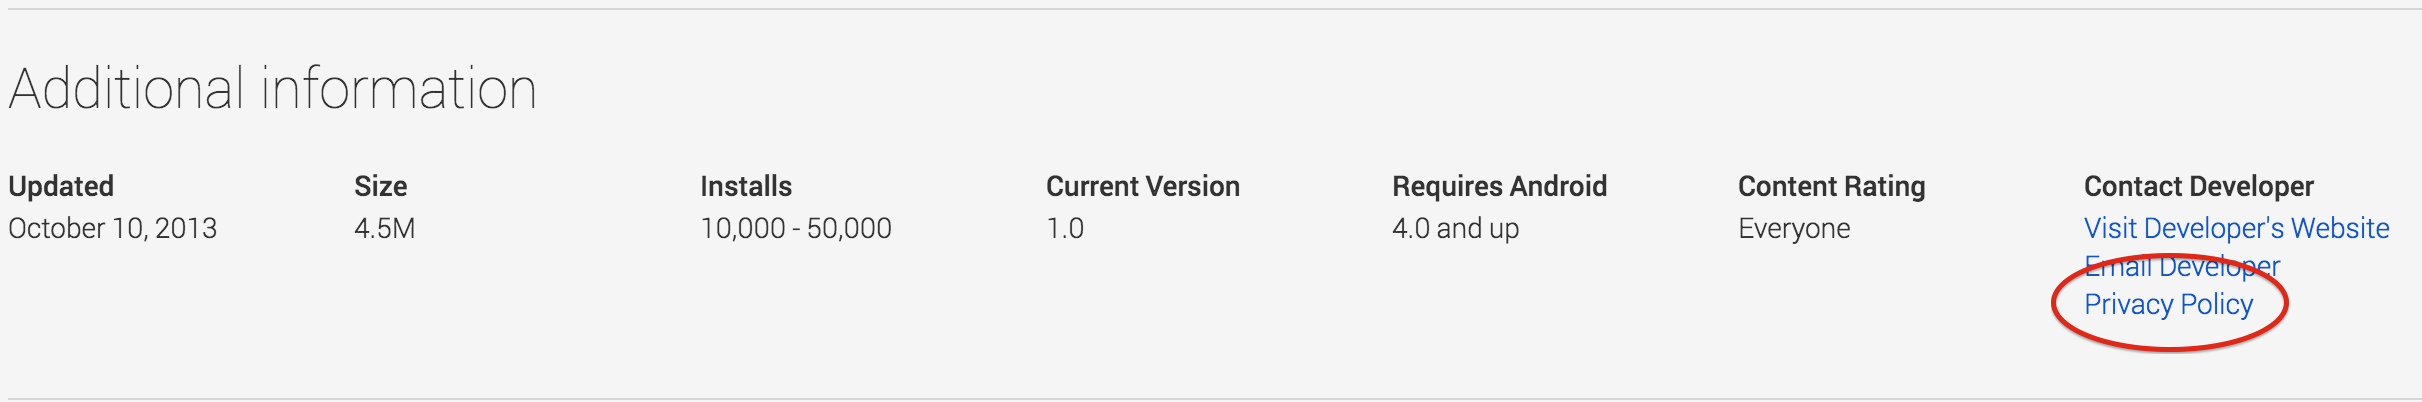
\includegraphics[width=\textwidth]{images/play-store-privacy-link}
      \caption{Privacy Policy link in the Play Store web interface}
      \label{fig:play-store-privacy-link}
\end{figure}

However, while the \texttt{AndroidManifest.xml} file is guaranteed to be present for any application on the Play Store, this does not hold true for the Privacy Policy link. 

In fact, no Play Store policies force an app to have a Privacy Policy at all.

So it can occur that either the app does not have a Privacy Policy at all, or that the developer has not inserted the Privacy Policy on the Play Store. In either case the automatic retrieval of the Privacy Policy of that app is impossible, so we will not further distinguish between them.

From the data we collected, it appears that out of the 1093 most downloaded free game apps, 39.79\% do not have a privacy policy publicly available through the Play Store.

% \todo[inline]{insert a pie chart here}

That being said, a Privacy Policy link does not guarantee the ability to retrieve an actual Privacy Policy document. The link can point to anything the developer decides, and this leads to extremely heterogeneous paths to reach the final document of our interest.

An example is redirection, which that is very common. As an example, the Privacy Policy URL for \emph{Angry Birds}, by Zynga, is:

\url{https://www.google.com/url?q=http://m.zynga.com/about/privacy-center/privacy-policy}

which redirects to

\url{http://m.zynga.com/about/privacy-center/privacy-policy}

which redirects to

\url{http://company.zynga.com/privacy/policy}

which contains the Privacy Policy document.

% \todo[inline]{Talk about the Disney example}

%%%%%%%%%%%%%%%%%%%%%%%%%%%%%%%%%%%%%%%%%%
\section{Semantic analysis}
Once the document has been retrieved, it needs to be semantically processed. For this purpose, we take advantage of Treat, a natural language processing framework for Ruby \cite{treat}. The Treat project aims to build a language-agnostic NLP framework for Ruby with support for tasks such as document retrieval, text chunking, segmentation and tokenization, natural language parsing, part-of-speech tagging, keyword extraction and named entity recognition.

The privacy policy document is firstly split into its logical subdivision using a SRX chunker, which implements the approach proposed in \cite{Milkowski:2009:USS:1987717.1987736}.

The the document is furthed split into sentences with the aid of a SRX segment, again following \cite{Milkowski:2009:USS:1987717.1987736}.


\begin{figure}[tb]
\centering
     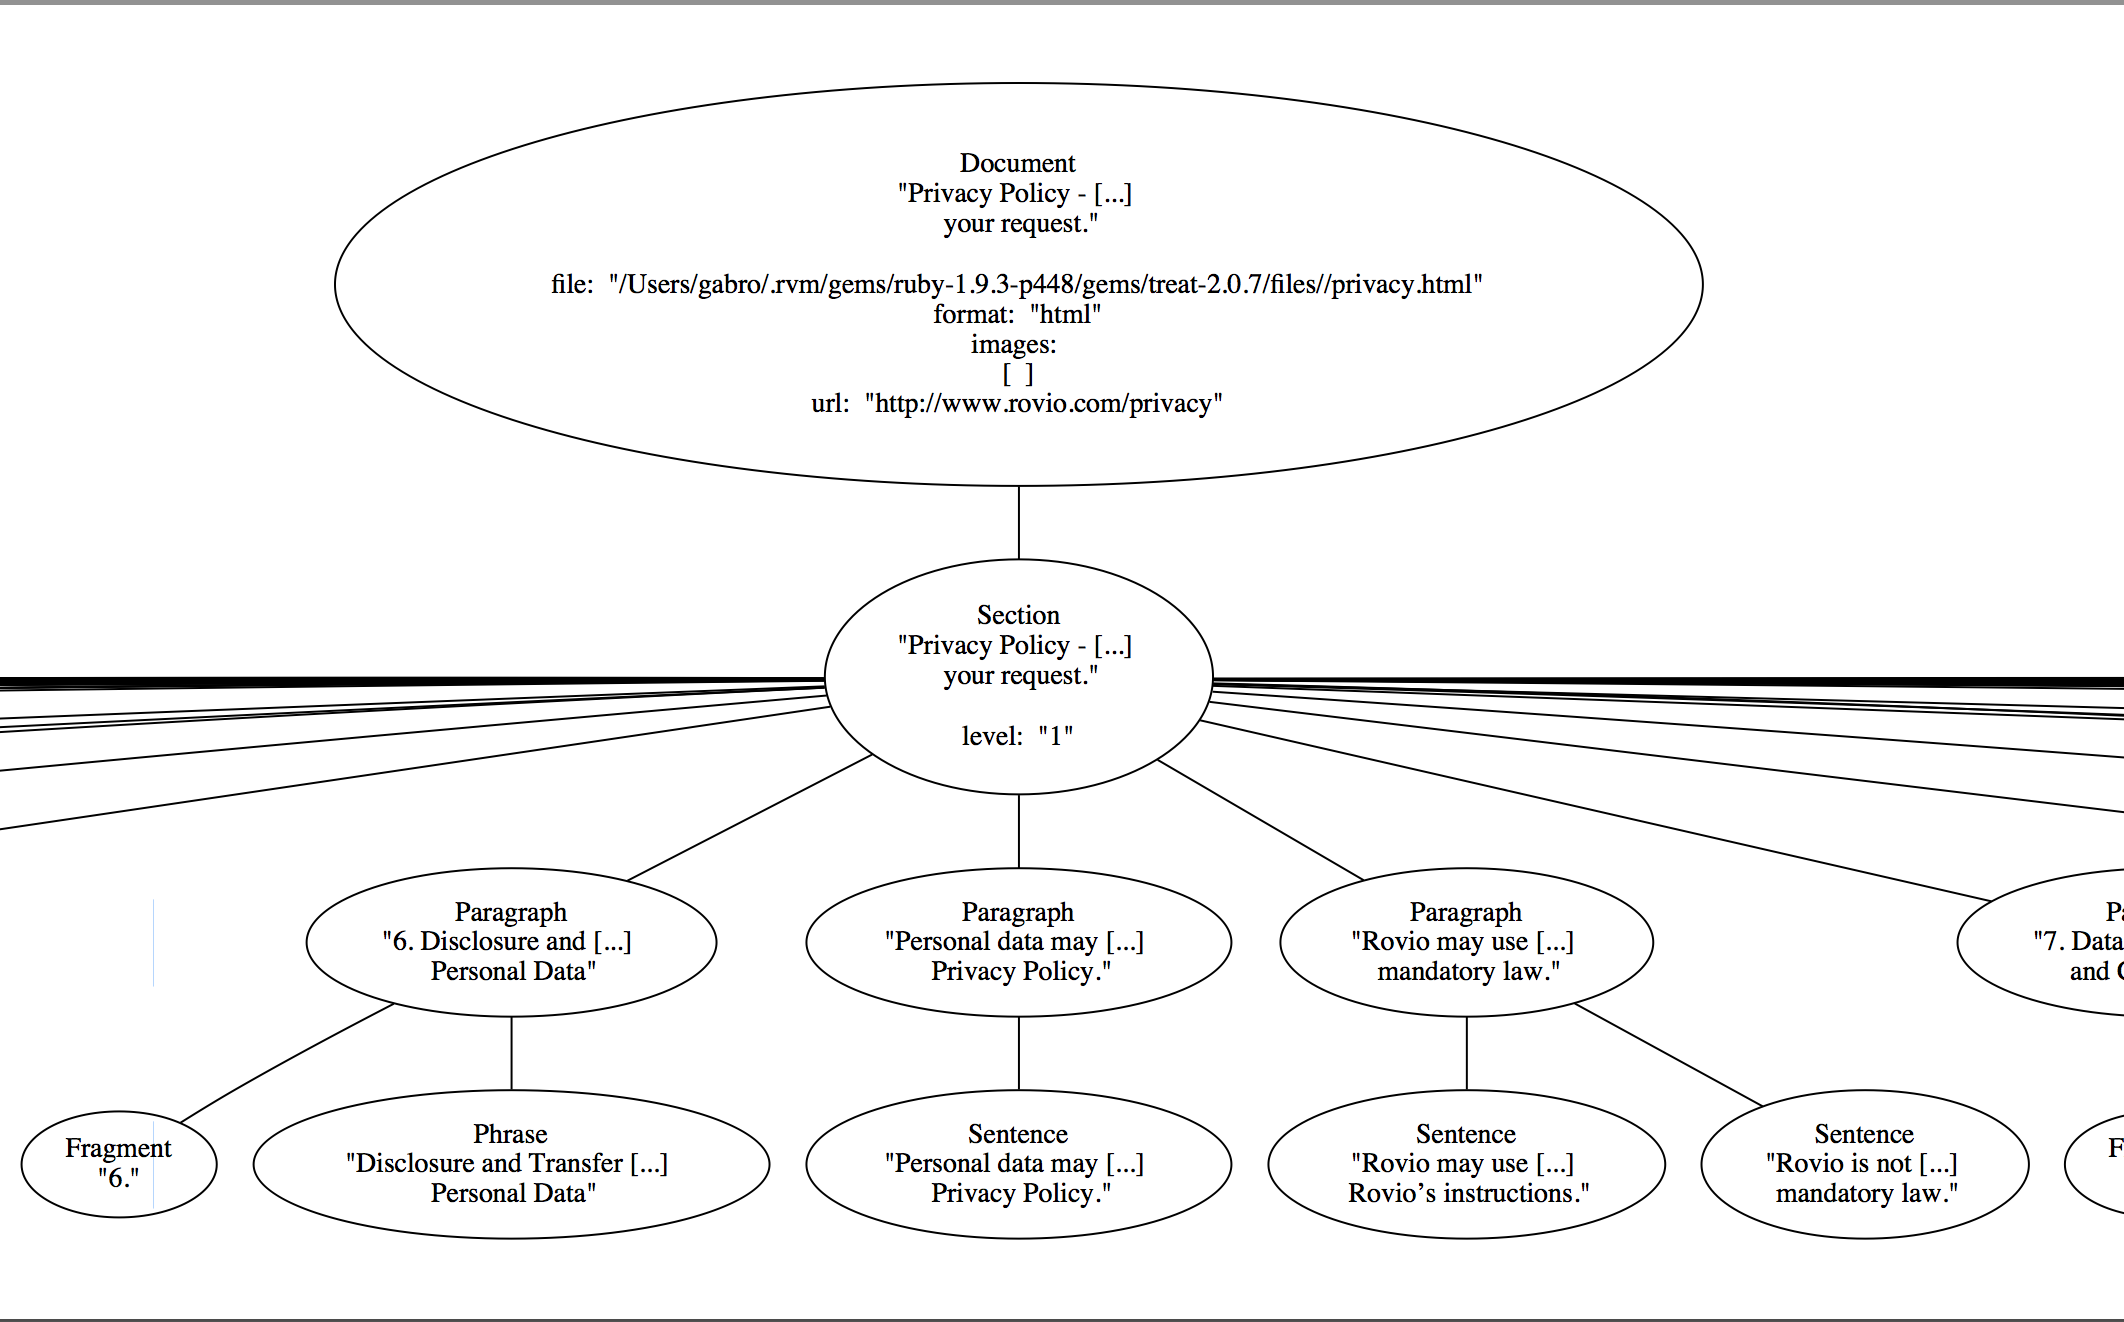
\includegraphics[width=\textwidth]{images/rovio-structure}
      \caption{Detail of Rovio's Privacy Policy structure}
      \label{fig:rovio-structure}
\end{figure}

\autoref{fig:rovio-structure} shows a detail of the semantic tree in which the original policy has been divided. Each internal node represents either paragraphs or sections of the document, whereas the leaf nodes are phrases and sentences.

Once sentences and phrases have been obtained, they can be searched for the expressions contained in the lookup table of each permission.
For example let us take the following sentence.

\begin{quote}
{\emph{``Rovio or third parties operating the ad serving technology may use demographic and \textbf{geo-location} information (for more information regarding use of Location Data see below Section 3) as well as information logged from your hardware or device to ensure that relevant advertising is presented within the Service.''}}\cite{rovio}
\end{quote}

The lookup table of \texttt{ACCESS\_COARSE\_LOCATION} contains the word ``location'', hence the above sentence will be matched and will be considered relevant to such permission.

\subsection{False positive detection}
As explained in \autoref{sec:false-positives}, we also need to search for `banned' verbal forms and exclude the sentences containing them. In order to be as general as possible, we want to consider every possible declination of the verb.
So the two main steps of this phase are:
\begin{itemize}
  \item identifying the verbs
  \item `normalizeing' each verb, in order to perform a comprehensive comparison
\end{itemize}

\subsubsection{Verb identification}
Identifying the verbs is achieved through \emph{part-of-speech tagging} (POS). POS, also called \emph{word-category disambiguation}, ``is the process of marking up a word in a text (corpus) as corresponding to a particular part of speech, based on both its definition, as well as its context—i.e. relationship with adjacent and related words in a phrase, sentence, or paragraph. A simplified form of this is commonly taught to school-age children, in the identification of words as nouns, verbs, adjectives, adverbs, etc.'' \cite{wiki:POS}. Different language taggers have been proposed over the last years: our choice fell on the most established one, i.e. the Stanford POS Tagger, which is a Java implementation of the log-linear POS tagger proposed in \cite{Toutanova:2003:FPT:1073445.1073478}.
Specifically we used the Ruby bindings provided by the aforementioned Treat framework.

As anticipated, the language tagger assigns a \emph{tag} to each word of a sentence; the tags used by the Standford Tagger are defined by the Penn Treebank tag set \cite{Marcus:1994:PTA:1075812.1075835}, in which we can find five different verb tags

\begin{itemize}
  \item VB:      Verb, base form
  \item VBD:     Verb, past tense
  \item VBG:     Verb, gerund or present participle
  \item VBN:     Verb, past participle
  \item VBP:     Verb, non-3rd person singular present
  \item VBZ:     Verb, 3rd person singular present 
\end{itemize}

Since we are interested in all the verbs of a sentence, we therefore consider all words with any of the above tags.

\subsubsection{Verbs normalization}
We are not really interested in the inflection of the verbs we are analyzing, rather we care about the concept they represent.
In order to catch all possible verbal forms, we make use of another feature of Treat: inflections. This feature allows us to perform a grammatical conjugation of an arbitrary verb.
Hence, we normalize all the verbs to their infinitive form before performing a comparison. For example, if we encounter a sentence containing the verb ``shipping'' and our ``false positive table'' includes the verb ``ship'', the sentence will be correctly excluded from the final result set.

\section{Results}
Results are discussed in detail in \autoref{sec:results}, however their collection brought up several technical challenges that required a rather sophisticated solution. The main issue is represented by the significant number of applications we want to analyze; for each one of them we need to retrieve their privacy policy, their permission list and then analyze such information.

The challenges then become:
\begin{itemize}
	\item Performing thousands of simultaneous requests to Play Store servers
	\item Performing thousands of simultaneous analysis on the same machine
\end{itemize}

The first challenge derives from Google's anti-bot protection, which results in an IP-ban in case of too many requests in a short amount of time.
The second challenges is instead an architectural limitation: spawning thousands of simultaneous computations easily hogs any personal computer's CPU, most likely leading to a system crash.

A naive approach to both challenges would be to serialize the operations, analyzing only one application at the time. However, considering an average processing time of 10 seconds per application, analyzing thousands of applications would require several hours of computation and such an architecture would not scale in case of an increased number of applications (e.g., if one would like to analyze a significant fraction of the Play Store).

What we want is then a fixed amount of computations running concurrently, in order to achieve a fast computation without hogging the computer's resources. We achieved this result taking a functional approach, namely utilizing Celluloid, a concurrent object oriented programming framework for Ruby.

Using Celluloid, we spawn a new computation for each thread - or in other terms, an \emph{actor} - which runs asynchronously and writes the results back to a MongoDB database. We use a fixed amout of actors, collectively referred to as a pool, in order to prevent the computation from using all of the computer resources, and also to prevent being banned from Google.
The result is a satisfying compromise between speed and available resources that allows to terminate the computation within reasonable time constraints.
	\chapter{Experimental Results}
		\label{chap:results}
		% !TEX root =  ../thesis.tex

In this chapter the results of our investigation are presented. We illustrate the quantitative results deriving from an automated analysis of several application on the Play Store; subsequently, we present a qualitative analysis and observation about the experiment.

\section{Quantitative results}
\label{sec:results}
In this section we present a metric used to evaluate the compliance of an application w.r.t. its privacy policy and we expose the quantitative results in terms of such metric.

\subsection{Metric definition}
\label{sec:metric}
First, we manually assign to each privacy-related permission a score from 1 to 3, representing the severity of its potential impact on the user's privacy, where 1 signifies a permission with low impact and 3 signifies a permission carrying a very high danger.

Such scores are defined by us, in accordance with observations and existing literature on permission analysis,
and are shown in \autoref{tab:permission-scores}.

\begin{table}[ht]
    \caption{PERMISSION IMPACT SCORES}
    \label{tab:permission-scores}
    \centering
    \begin{tabular}{clc}
        \toprule
            \#   & Permission impact scores \\
            \midrule
                1  & INTERNET                       &   3 \\
                2  & READ\_EXTERNAL\_STORAGE        &   2 \\
                3  & WRITE\_EXTERNAL\_STORAGE       &   2 \\
                4  & ACCESS\_WIFI\_STATE            &   1 \\
                5  & READ\_PHONE\_STATE             &   3 \\
                6  & GET\_ACCOUNTS                  &   3 \\
                7  & ACCESS\_COARSE\_LOCATION      	&   3 \\
                8  & GET\_TASKS                     &   1 \\
                9  & ACCESS\_FINE\_LOCATION         &   3 \\
                10 & READ\_LOGS                     &   1 \\
                11 & RECORD\_AUDIO                  &   2 \\
                12 & READ\_CONTACTS                 &   3 \\
        \bottomrule
    \end{tabular}
\end{table}

Secondly, we use the scores to compute a weighted sum of the number of permissions that lack an explicit mention in the privacy policy.

\begin{align}
\label{eq:goodness-metric}
	\sum\limits_{i=1}^n &= w_i p_i \\
	w_i &= \text{ score of the} i^{th} \text{permission} \\
	%
	p_i &=
	\begin{cases}
		& 0 \text{ if the permission is mentioned in the privacy policy} \\
		& 1 \text{ otherwise}
	\end{cases}
\end{align}

The final result is a metric estimating the compliance of an Android application to its own privacy policy. The lower the score, the more compliant the application.

We the analysis on the same 4300 applications used to generate the list of most used permissions, and the results are shown in \autoref{fig:results}

\begin{figure}[t]
\centering
     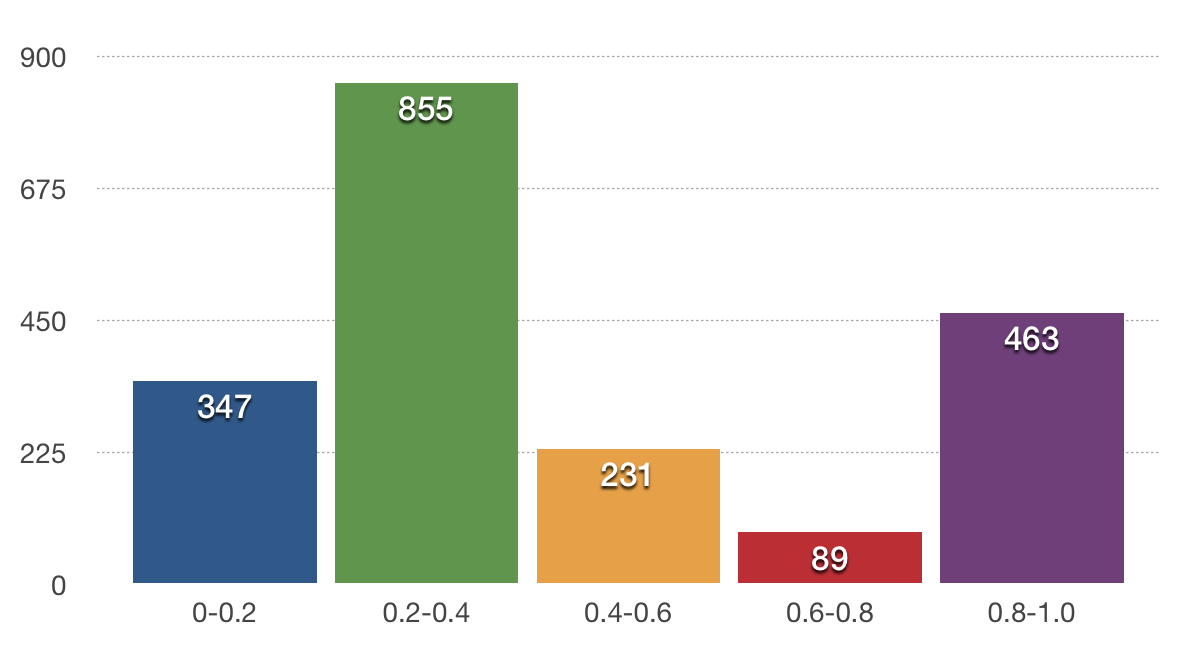
\includegraphics[width=0.9\textwidth]{images/results}
      \caption{Quantitative results (over 4300 applications, December 7, 2013)}
      \label{fig:results}
\end{figure}

\section{Qualitative results}
\label{sec:qualitative-results}
Out of the thousands of applications analyzed, we now focus our attention on a few notable cases.

\section{Case study: Shopkick}
Shopkick is a popular shopping rewards app and is known \cite{shopkick-lifehacker} to require some sensitive permissions that should worry any user of this app. \autoref{tab:shopkick-permissions} shows the complete list of permissions of the Android application.

\begin{table}[ht]
    \caption{SHOPKICK APP PERMISSIONS}
    \label{tab:shopkick-permissions}
    \centering
    \begin{tabular}{l}
        \toprule
            Permissions \\
            \midrule
                INTERNET \\
                ACCESS\_NETWORK\_STATE \\
                ACCESS\_COARSE\_LOCATION \\
                ACCESS\_FINE\_LOCATION \\
                READ\_PHONE\_STATE \\
                WRITE\_EXTERNAL\_STORAGE \\
                ACCESS\_WIFI\_STATE \\
                RECORD\_AUDIO \\
                CAMERA \\
                FLASHLIGHT \\
                VIBRATE \\
                BLUETOOTH \\
                GET\_ACCOUNTS \\
                RECEIVE\_BOOT\_COMPLETED \\
                READ\_CONTACTS \\
                CALL\_PHONE \\
                WAKE\_LOCK \\
                READ\_EXTERNAL\_STORAGE \\
                READ\_CALL\_LOG \\
        \bottomrule
    \end{tabular}
\end{table}

We can immediately spot a few permissions with a very high impact score, for example \texttt{RECORD\_AUDIO}, \texttt{CAMERA} and \texttt{ACCESS\_FINE\_LOCATION}.

\texttt{RECORD\_AUDIO} grants the application the ability to access the device microphone to record audio, without any explicit consent by the user other than installing the app itself. This means that the app is virtually enabled to record audio at any time, with no possibility of being disabled. Especially in combination with the \texttt{RECEIVE\_BOOT\_COMPLETED} permission, which allows the app to be launched when the phone has booted, and the \texttt{INTERNET} permission, which enables sending data over the Internet, this is considerably worrying: the application could easily start itself as soon as the phone has been turned on, constantly record any sound going through the device's microphone and finally send everything over the Internet to a remote server, where the content can be stored and accessed in a later time.

To make things worse, the application also requests the permission \texttt{ACCESS\_FINE\_LOCATION}, meaning that the audio recording can be triggered according to the user's location, perhaps the workplace, home or other sensitive locations.

It is not hard to see how these capabilities can turn the app into a roving spyware, i.e. an application with whose hidden purpose is eavesdropping and spying on the device owners, as well as the people they have contacts with.

Further investigations reveal how the app apparently uses the device's microphone in order to validate the physical location of the user in a store. According to the New York Times, \emph{``The app knows someone is in a store by listening for an audio transmitter placed in each participating store; the phone's microphone picks up the signal, which people cannot hear.''}\cite{shopkick-nyt}.

We can formalize a subset of this situation in terms of the representation previously discussed in \autoref{chap:intro}.
\begin{itemize}
    \item The permission \texttt{RECORD\_AUDIO} ($P_1$) enables the action \\ \emph{record\_audio\_from\_the\_device\_microphone} ($A\_1$);
    \item the permission \texttt{INTERNET} ($P\_2$) enables the action \\ \emph{send\_data\_over\_the\_internet} ($A\_2$);
    \item the permission \texttt{CAMERA} ($P\_3$) enables the action \\ \emph{record\_images\_from\_the\_device\_camera} ($A\_3$);
    \item the permission \texttt{ACCESS\_FINE\_LOCATION} enables the action \\ \emph{detect\_location\_of\_device} ($A_4$)
\end{itemize}

The combination of $A_1$ and $A_2$ enables the behavior \emph{validate\_presence\_in\_store} ($B\_1$). On the other hand $A\_1$, $A\_2$, $A\_3$ and $A\_4$ can also be combined enabling the behavior \emph{record\_audio\_and\_video\_when\_user\_is\_at\_home} ($B_2$).

Both behaviors are unexpected to the user, but while $B_1$ is probably considered legit - and even desirable -, $B_2$ is definitely unexpected, undesirable, and possibly unlawful.

We now look at Shopkick's privacy policy looking for references of the aforementioned permissions.

\subsection{RECORD}
Our tool identifies this paragraph as relevant to the matter of recording audio:

\begin{quote}
{\emph{``(iv) record, determine or use information about or from another content delivery platform (for example, to unlock potential rewards or offers based on your watching of a specific a commercial or show that is broadcast on your television or on the web, the shopkick application may ask you to open the app while you are watching TV, and then \textbf{we may record or analyze the audio signal from the television set via the shopkick app and your cell phone's microphone}, to determine the commercial, and/or program, including the date and/or time)''}}\cite{shopkick}
\end{quote}

A manual inspection of the policy confirms that this is indeed the relevant section and that the permissions are covered by the privacy policy.

\subsection{ACCESS\_FINE\_LOCATION}
Concerning the user's location, the tool identifies this sentence as relevant:

\begin{quote}
{\emph{(i) automatically record information that your mobile phone/device sends or transmits, including […] geographical location (if you consent to that)}}
\end{quote}

While it is true that the privacy policy covers this matter, it is also worth noting how the last phrase is misleading: as we saw before, the user grants permissions at install time on an Android device, so the consensus has already been given. Stating \emph{If you consent to do that} gives a sense of false assurance.

\subsection{CAMERA}
The tool signals that no references have been found in the privacy policy regarding the \texttt{CAMERA} permission and a manual inspections confirms that Shopkick's privacy policy doesn't mention in any way the use of the device's camera as a medium of acquiring data.

As it currently stands, Shopkick's application can collect any image from the user's camera without they being notified and the privacy policy does not restrict this by any mean.

Our tool successfully detected this behavior, helping in identifying a gap in the privacy policy of this popular application.
	\chapter{Conclusions and Future Work}
		\label{chap:conclusion}
		% !TEX root =  ../thesis.tex

We presented a novel approach to the analysis of privacy policies in the context of Android applications. We introduced a framework for reasoning and proving properties of privacy policies, laying down the foundation for a new area of investigation.

The tool we implemented greatly eases the process of understanding the privacy implications of installing third party apps and it has already been proven able to highlight worrisome instances of applications.

The tool is developed with expandability in mind, and further developments in the approach can easily be integrated in order to increase the reliability and effectiveness.

This thesis aims at laying the foundation for a new area of investigation, namely the relationship between mobile applications capabilities and behaviors and their privacy policies. As we mentioned in \autoref{chap:intro} several steps can be taken towards user awareness about privacy matters and this work covers the first necessary ones: identifying and analyzing the privacy-relevant permissions and examining their relationships with the privacy policies language. This enables further steps in the investigation and we now outline some of them.

As anticipated in \autoref{chap:intro}, the first natural steps following the present work would be to live monitor the application's behavior. A static analysis can provide useful information about the \emph{potential} behaviors that can occur, but only a dynamic observation of applications running on real device can give insights about the \emph{actual} behaviors.

The first implementation one can think of is a passive monitoring of applications, with the final purpose of reporting such behaviors and further refine the ``goodness'' score presented in \autoref{sec:metric}.

One can also think of taking a step further and turn the monitoring into an active defense: if the application is found performing a behavior clearly in contrast with its privacy policy, the monitoring tool can immediately inform the user or even prevent such behavior from happening.

As discussed in \autoref{sec:false-positives}, the proposed approachoccasionally incurs in false positives and we illustrated a possible solution to this issue based on verb detection.

As anticipated, another viable solution is to allow the users of the tool to provide feedback on each sentence. They could either mark the sentence as \emph{relevant} or \emph{not relevant} and therefore improve the scoring of an application.

The same approach could then be used to identify false negatives: relevant sentences can be not recognized and a user can signal such fact indicating which relevant portions of the privacy policy apply to the selected permission.

	% \begin{appendices}
	% 	\chapter{Lookup tables}
	% 	\label{app:a}
	% 	% !TEX root =  ../thesis.tex
\begin{table}[tbh]
    \caption{ACCESS\_COARSE\_LOCATION LOOKUP TABLE}
    \label{tab:lookup-coarse-location}
    \centering
    \begin{tabular}{lp{6cm}}
        \toprule
            Permission   & Keywords \\
            \midrule
                \texttt{ACCESS\_COARSE\_LOCATION}  & \emph{``gps''}, \emph{``IP based location''}, \emph{``location''}, \emph{``location services''}, \emph{``geo-location''}, \emph{``geographic location''} \\
        \bottomrule
    \end{tabular}
\end{table}

\begin{table}[tbh]
    \caption{RECORD\_AUDIO LOOKUP TABLE}
    \label{tab:lookup-record-audio}
    \centering
    \begin{tabular}{lp{9cm}}
        \toprule
            Permission   & Keywords \\
            \midrule
                \texttt{RECORD\_AUDIO}  & \emph{``microphone''}, \emph{``record audio''}, \emph{``record voice''}, \emph{``audio''} \\
        \bottomrule
    \end{tabular}
\end{table}
	% \end{appendices}

	\clearpage
	\phantomsection
	\bibliographystyle{plain}
	\bibliography{thesis}
	\nocite{*}

	% \newpage
	% \phantomsection
	% % !TEX root =  ../thesis.tex
\vita

\begin{center}
\begin{singlespace}

{\Huge Gabriele Petronella}

\vspace{0.4in}

\begin{tabular}{r@{\hspace{0.2in}}|@{\hspace{0.2in}}p{3.8in}}

{\Large Education}
& \textbf{B.S., Engineering of Computing Systems} \\
& Politecnico di Milano \\
& 2011 \\
\\
& \textbf{M.S., Computer Science (\emph{current})} \\
& University of Illinois at Chicago, Chicago, IL \\
& 2013 \\
\\

{\Large Working experience}
& \textbf{Co-founder} \\
& \emph{Metwit Ltd}  \small{2011-2012}\\ 
& Dubai, UAE - London, UK \\
& Founded a crowdsourced weather startup and lead the develpment of the iOS client. \\
\\

& \textbf{Co-founder} \\
& \emph{buildo s.r.l.s.}  \small{2013-present}\\ 
& Milan, Italy \\
& Software architect and developer. \\
\\

& \textbf{Research Assistant} \\
& \emph{University of Illinois at Chicago} \small{Sept 2012-Dec 2013} \\
& Chicago, IL \\
& Research activity focused on privacy policies formal analysis.
\end{tabular}

\end{singlespace}
\end{center}

\end{document}
